Suppose we have a set of pre-classified data points $x_i$ in $\mathbb{R}^n$, divided into two sets based on their classification. For example, the data could be information on patients and the two sets would correspond to patients who have or do not have a certain disease. Note that unlike so far, $x$ is now data, not a decision variable. Denote the respective index sets by $I_1$ and $I_2$, respectively. In order to predict the class of a new point $x_{new}$, we want to infer a classification rule from the data.
\begin{figure}
    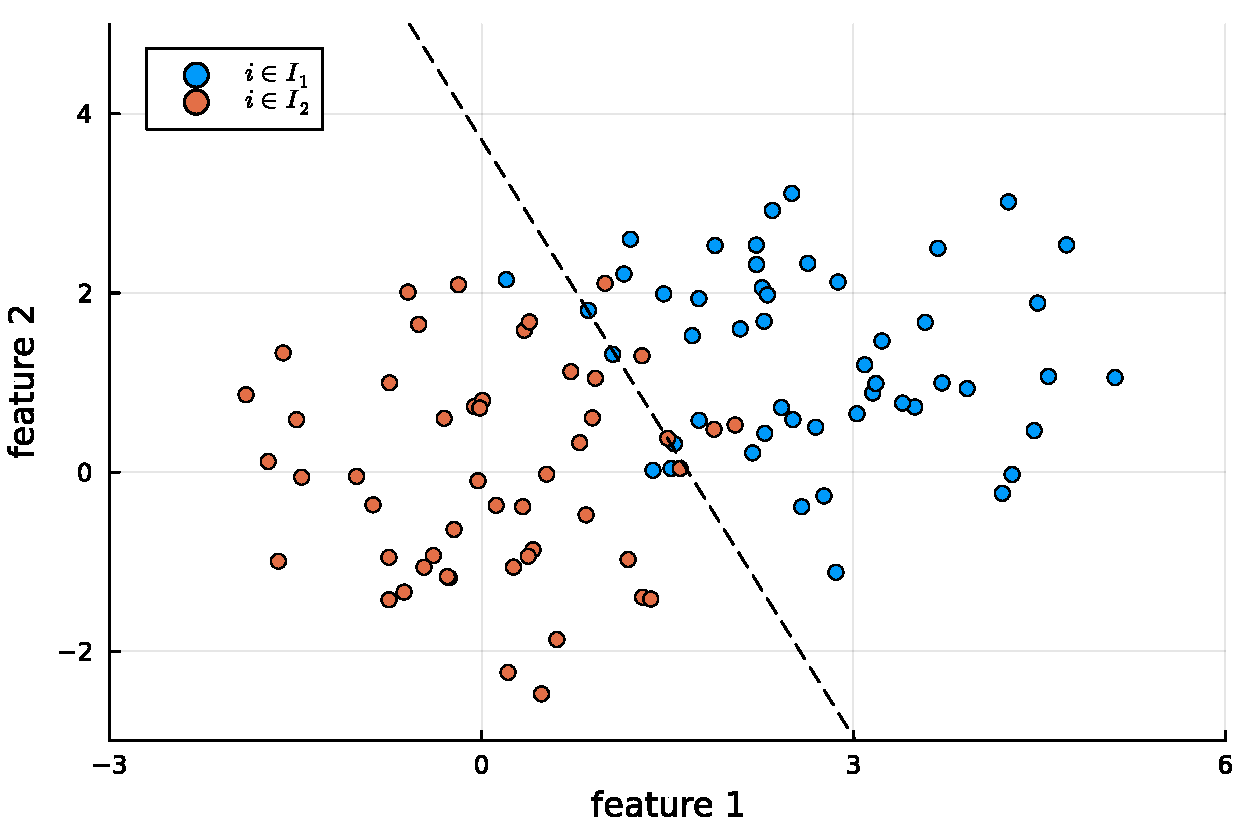
\includegraphics[width=0.75\textwidth]{part_1/chapter_1/figures/figure_e16.pdf}
    \caption{Two sets of data points defined by two features, separated by a line $ax=b$} \label{p1c1:fig:fig_e16}		
\end{figure}

Write a linear programming problem that finds the hyperplane $ax = b$ minimizing the sum of absolute deviations $|ax_i-b|$ for the misclassified points $x_i$, that is, points on the wrong side of the hyperplane. In Fig. \ref{p1c1:fig:fig_e16}, any red point $x_i$, $i \in I_2$ that is on the top/right of the line is on the wrong side and thus accumulates the error, and similarly for blue points on the bottom/left of the line.
